\documentclass{article}
\usepackage[english]{babel}
\usepackage{amsmath,graphicx}

%%%%%%%%%% Start TeXmacs macros
\newcommand{\tmtextbf}[1]{\text{{\bfseries{#1}}}}
%%%%%%%%%% End TeXmacs macros

%


\begin{document}

\title{Connexion entre Impulsion, Fr{\'e}quence et Longueur d'Onde}

\date{April 29, 2025}

\maketitle

\section*{1. Cas du Photon (masse nulle)}

\begin{itemize}
  \item \tmtextbf{{\'E}nergie du photon} : $E = hf$
  
  \item \tmtextbf{Impulsion du photon} : $p = \frac{hf}{c}$
  
  \item \tmtextbf{Longueur d'onde} : $\lambda = \frac{c}{f}$
  
  \item \tmtextbf{Relation de De Broglie} : $p = \frac{h}{\lambda}$
\end{itemize}
\begin{figure}[h]
  \begin{center}
    \resizebox{0.8\columnwidth}{!}{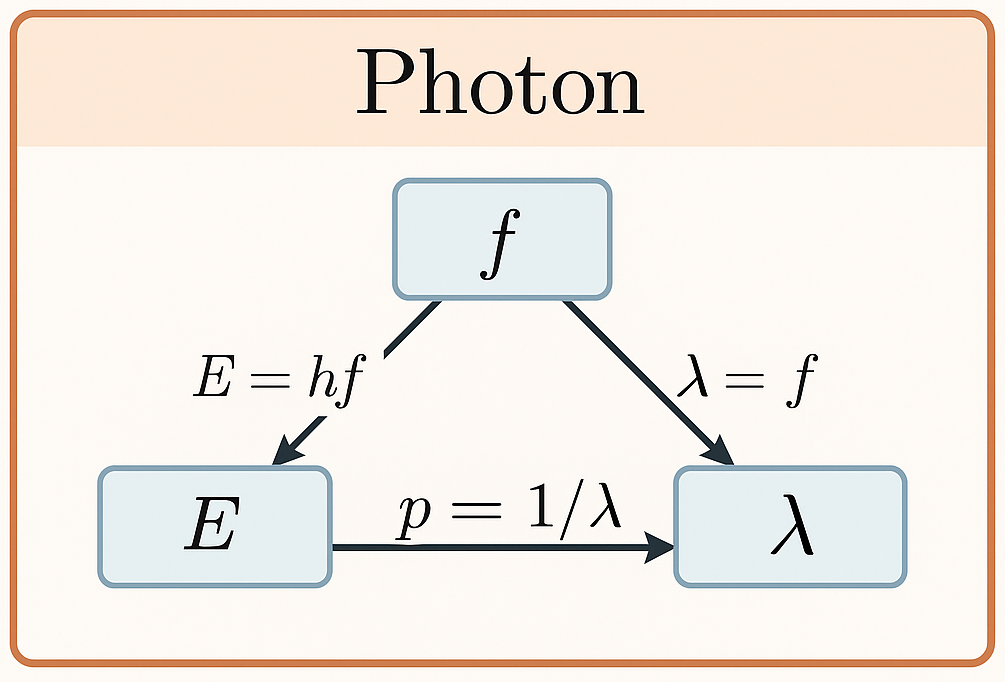
\includegraphics{photon.png}} 
  \end{center}
  \caption{Relations fondamentales pour un photon}
\end{figure}

\section*{2. Cas de l'{\'E}lectron (masse non nulle)}

\begin{itemize}
  \item \tmtextbf{Impulsion} : $p = mv$
  
  \item \tmtextbf{Longueur d'onde de De Broglie} : $\lambda = \frac{h}{mv}$
  
  \item \tmtextbf{Cas relativiste} : $E^2 = (pc)^2 + (m_0 c^2)^2$
\end{itemize}
\begin{figure}[h]
  \begin{center}
    \resizebox{0.6\columnwidth}{!}{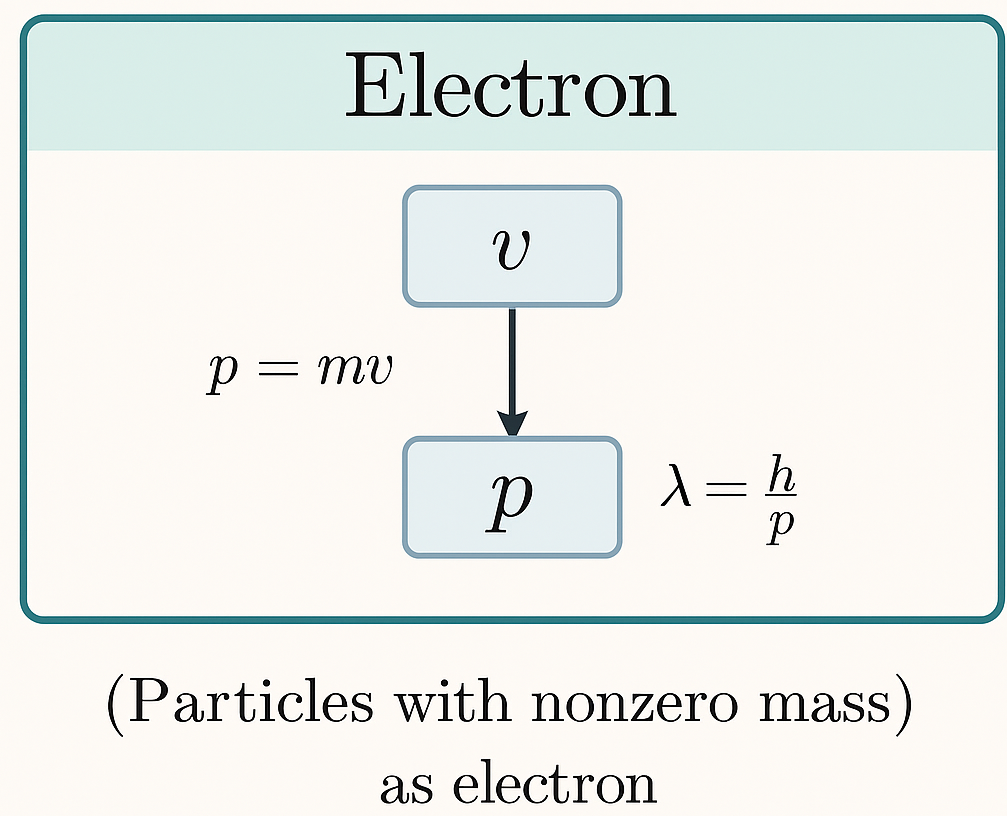
\includegraphics{electron.png}} 
  \end{center}
  \caption{Relations pour une particule massive comme l'{\'e}lectron}
\end{figure}

\section*{3. Synth{\`e}se}

\begin{center}
  \begin{tabular}{|c|c|c|c|}
    \hline
    \tmtextbf{Particule} & \tmtextbf{{\'E}nergie} & \tmtextbf{Impulsion $p$} &
    \tmtextbf{Longueur d'onde $\lambda$}\\
    \hline
    Photon & $E = hf$ & $p = \frac{hf}{c}$ & $\lambda = \frac{c}{f}$\\
    \hline
    {\'E}lectron (non relativiste) & $E = \frac{1}{2} mv^2$ & $p = mv$ &
    $\lambda = \frac{h}{mv}$\\
    \hline
  \end{tabular}
\end{center}

\end{document}
